\documentclass[12pt]{article} % 12pt 为字号大小 UTF8
\usepackage{amssymb,amsfonts,amsmath,amsthm}
%\usepackage{fontspec,xltxtra,xunicode}
%\usepackage{times}

%----------
% 定义中文环境
%----------

\usepackage{xeCJK}
\usepackage{booktabs}
\usepackage{multirow}
\usepackage{url}
% \setCJKmainfont[BoldFont={SimHei},ItalicFont={KaiTi}]{SimSun}
% \setCJKsansfont{SimHei}
% \setCJKfamilyfont{zhsong}{SimSun}
% \setCJKfamilyfont{zhhei}{SimHei}

% \newcommand*{\songti}{\CJKfamily{zhsong}} % 宋体
% \newcommand*{\heiti}{\CJKfamily{zhhei}}   % 黑体


%----------
% 版面设置
%----------
%首段缩进
\usepackage{indentfirst}
\setlength{\parindent}{2.1em}

%行距
\renewcommand{\baselinestretch}{1.4} % 1.4倍行距

%页边距
\usepackage[a4paper]{geometry}
\geometry{verbose,
  tmargin=3cm,% 上边距
  bmargin=3cm,% 下边距
  lmargin=3cm,% 左边距
  rmargin=3cm % 右边距
}


%----------
% 其他宏包
%----------
%图形相关
\usepackage[x11names]{xcolor} % must before tikz, x11names defines RoyalBlue3
\usepackage{graphicx}
\usepackage{pstricks,pst-plot,pst-eps}
\usepackage{subfig}
\def\pgfsysdriver{pgfsys-dvipdfmx.def} % put before tikz
\usepackage{tikz}

%原文照排
\usepackage{verbatim}

%网址
\usepackage{url}

%----------
% 习题与解答环境
%----------
% %习题环境
% \theoremstyle{definition} 
% \newtheorem{exs}{习题}

% %解答环境
% \ifx\proof\undefined\
% \newenvironment{proof}[1][\protect\proofname]{\par
% \normalfont\topsep6\p@\@plus6\p@\relax
% \trivlist
% \itemindent\parindent
% \item[\hskip\labelsep
% \scshape
% #1]\ignorespaces
% }{%
% \endtrivlist\@endpefalse
% }
% \fi

% \renewcommand{\proofname}{\it{证明}}

%----------
% 我的自定义
%----------

\newcommand{\horrule}[1]{\rule[0.5ex]{\linewidth}{#1}} 	% Horizontal rule

\renewcommand{\refname}{参考文献}
\renewcommand{\abstractname}{\large \bf 摘\quad 要}
\renewcommand{\contentsname}{目录}
\renewcommand{\tablename}{表}
\renewcommand{\figurename}{图}

\setlength{\parskip}{0.4ex} % 段落间距

\usepackage{enumitem}
\setenumerate[1]{itemsep=0pt,partopsep=0pt,parsep=\parskip,topsep=5pt}
\setitemize[1]{itemsep=0.4ex,partopsep=0.4ex,parsep=\parskip,topsep=0.4ex}
\setdescription{itemsep=0pt,partopsep=0pt,parsep=\parskip,topsep=5pt}


%==========
% 正文部分
%==========

\begin{document}

\title{
{\normalfont\normalsize\textsc{
Lanzhou University\\
Computer Organization, Autumn 2022 \\[25pt]}}
\horrule{0.5pt}\\
\sffamily{计算式组成原理\\单周期CPU设计}
\horrule{1.8pt}\\[20pt]
}
\author{王天一,tianyiwang58@gmail.com\\
	王天志,wangtzh20@lzu.edu.cn\\
	聂嘉一,niejy20@lzu.edu.cn\\
	叶清扬,yeqy20@lzu.edu.cn}
\date{2022年4月} % 若不需要自动插入日期,则去掉前面的注释;{ } 中也可以自定义日期格式

\begin{titlepage}
\maketitle
\vspace{30pt}
\begin{abstract}
\normalsize \ \ 在这次作业中,我们设计了一个基于MIPS指令集的单周期CPU。并对于我们的成品,进行了进一步验证: \\
\ \ \textbf{1)} 进行了功能前仿.\\
\ \  \textbf{2)} 测试了性能指标(频率、已实现指令的条数和CPI) 。\\
\ \ \textbf{3)}交叉编译简单的C程序,使用MARS运行测试。\\
\ \ \textbf{4)}使用了FPGA静态存储器(俗称IP核)存储机器指令。\\[5pt]
\indent \ \ \textbf{关键词}:CPU,Verilog, 计算机组成原理
\end{abstract}
\thispagestyle{empty}
\end{titlepage}

\tableofcontents
\thispagestyle{empty}

\newpage
\setcounter{page}{1}

\section{引言}
这个模板是UTF-8编码的,使用xeCJK宏包,中英文混排更美观,但编译速度稍慢。注意:该模板只能用xelatex编译。本模板支持Overleaf在线\LaTeXe 平台,网址:\url{https://www.overleaf.com}。详细的\LaTeX 使用方法这里不详细展开,仅列举一些常用的。

引言也称前言、序言或概述,作为科技论文的开端,提出文中要研究的问题,引导读者阅读和理解全文。


\section{指令集}
对于指令集,我们参考了MIPS指令集共实现了\textbf{31}条指令集,其中包括\textbf{17}条R型指令,\textbf{12}条i型指令,\textbf{2}条J型指令。%这里加一个ref  https://blog.csdn.net/yixilee/article/details/4316617

\subsection{段落}
正文会有大量的文字段落。假设这是一个很长的段落,假设这是一个很长的段落,假设这是一个很长的段落,假设这是一个很长的段落,假设这是一个很长的段落,假设这是一个很长的段落,假设这是一个很长的段落,假设这是一个很长的段落,假设这是一个很长的段落,假设这是一个很长的段落,假设这是一个很长的段落,假设这是一个很长的段落,假设这是一个很长的段落,假设这是一个很长的段落。

这是下一段。假设这是一个很长的段落,假设这是一个很长的段落,假设这是一个很长的段落,假设这是一个很长的段落,假设这是一个很长的段落,假设这是一个很长的段落,假设这是一个很长的段落,假设这是一个很长的段落,假设这是一个很长的段落,假设这是一个很长的段落,假设这是一个很长的段落。

这是另一段

这又是一段。

这是最后一段,它由好多好多非常多多好多非常多多好多非常多多好多非常多多好多非常多多好多非常多多好多非常多多好多非常多多好多非常多的条目组成,就像下面这个样子:

\begin{itemize}
  \item 这里引用了一篇文献\cite{cao17}。
  \item 这是一个很长很长很长很长很长很长很长很长很长很长很长很长很长很长很长很长很长很长很长很长很长很长很长很长很长很长很长很长很长很长很长很长很长很长很长很长很长很长很长很长很长很长很长很长的条目。
\end{itemize}

\subsection{字体}
默认字体为宋体。{\sffamily 这是黑体。} {\rmfamily 这是宋体。} {\ttfamily 这是仿宋。} {\it 这是楷体。}
或者\textsf{黑体},\textrm{宋体},\texttt{仿宋},\textit{楷体}。

\subsubsection{文字强调}
加粗宋体:\textbf{粗体},加斜字体自动变成楷体:\textit{强调}。

更多中文说明(网址有点长,显示不全):\\\url{https://www.overleaf.com/latex/examples/using-the-ctex-package-on-overleaf-zai-overleafping-tai-shang-shi-yong-ctex/gndvpvsmjcqx/viewer.pdf}

\subsubsection{子小节}
这是另一个子小节。

\subsection{公式}
\begin{equation}
\label{eqn:eqn1}
\mathbf{A}=\sum\limits_{i=0}^{N-1}{e^{j\frac{2\pi}{N}i}}=0
\end{equation}

\subsection{定理}
正文中可能有很多定理、定义、证明、引理等等。这一特性目前可以手动实现和标号,以后会添加自动方法。


\section{实验}
实验中存在大量图表。实验中存在大量图表。实验中存在大量图表。实验中存在大量图表。实验中存在大量图表。实验中存在大量图表。实验中存在大量图表。实验中存在大量图表。实验中存在大量图表。实验中存在大量图表。实验中存在大量图表。实验中存在大量图表。实验中存在大量图表。实验中存在大量图表。实验中存在大量图表。实验中存在大量图表。实验中存在大量图表。实验中存在大量图表。实验中存在大量图表。实验中存在大量图表。实验中存在大量图表。实验中存在大量图表。实验中存在大量图表。实验中存在大量图表。实验中存在大量图表。实验中存在大量图表。实验中存在大量图表。实验中存在大量图表。实验中存在大量图表。下面演示图表的用法。

\subsection{图}
\begin{figure}[ht]
\centering
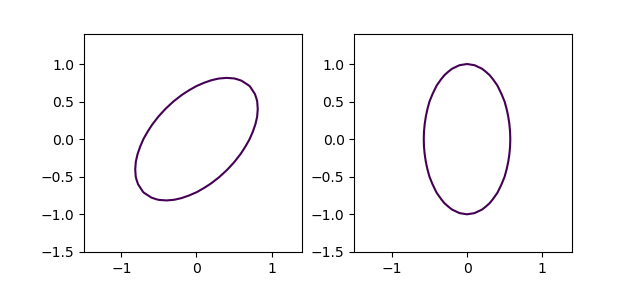
\includegraphics[width=\textwidth]{canoform.png}
\caption{这是一个图}
\label{fig:fig1}
\end{figure}
引用图\ref{fig:fig1} 。

\subsection{表}
\begin{table}[ht]
\caption{这是一个表}
\label{tb:filter}
\centering
\begin{tabular}{cccc}
\hline
 & 卡尔曼滤波 & 神经网络滤波 & 被动无源滤波 \\ 
\hline
模型类型 & 线性 & 线性 & 非线性 \\ 
参数调校 & 大量 & 几乎没有 & 合理 \\ 
稳定性 & 满足全局稳定性 & 依赖于模型 & 满足子系统稳定性 \\ 
\hline
\end{tabular} 
\end{table}
引用表格\ref{tb:filter} 。

\section{性能指标分析}
\subsection{CPI}
参考课件,我们可以知道,CPI计算公式为
$$
CPI = \frac{\mbox{CPU时钟周期数}}{\mbox{指令条数}} 
$$
显而易见,在我们的单周期CPU上,一个时钟周期只运行一条指令,因此我们可以计算出$CPI = 1$。
\subsection{等效频率}
参考课件,我们可以知道等效频率的计算公式为
$$
\mbox{等效频率} = \frac{1}{\mbox{时钟频率}}
$$
\section{代码实现}
\section{数据通路}
\section{加分项一}
使用C语言编写简单程序,覆盖到CPU所支持的分指令,使用MIPS或RISCV交叉编译(mips-linux-gcc或gcc-riscv)为汇编源码,使用MIPS或RISCV模拟器翻译为机器指令并执行,加0-15分。
\subsection{技术实现}
这里我们测试的代码为优化过的递归版斐波那契数列,代码详见图 \ref{fig:ExtraProCSource1}。
\begin{figure}[ht]
	\centering
	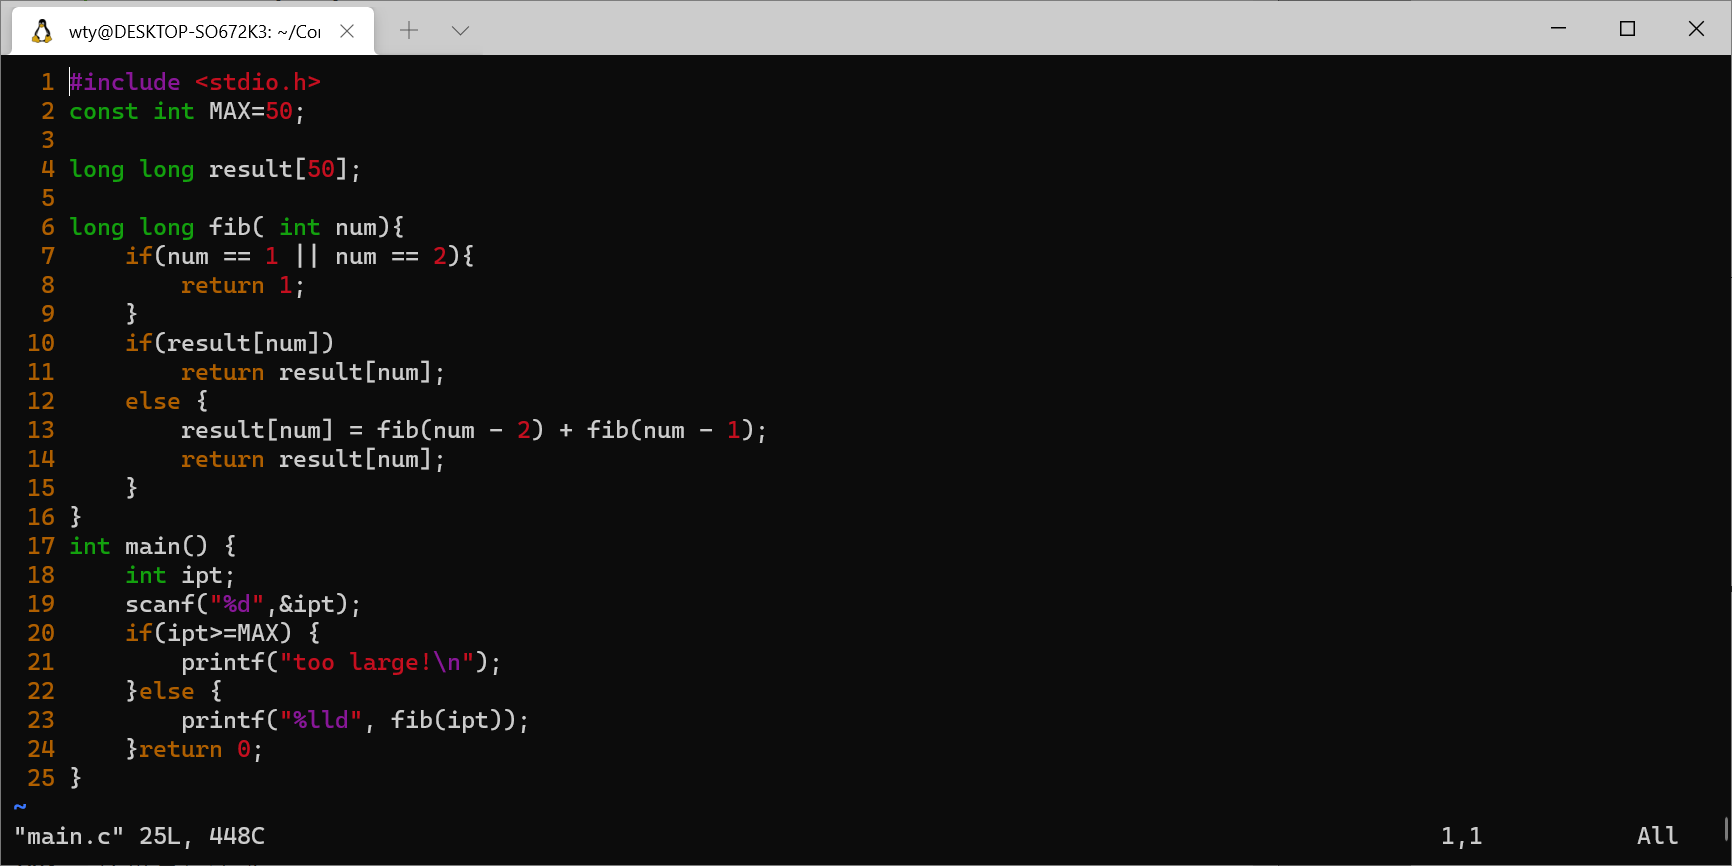
\includegraphics[width=\textwidth]{figures/figure1.png}
	\caption{加分项一C语言源代码}
	\label{fig:ExtraProCSource1}
\end{figure}
然后我们使用mips-linux-gcc工具交叉编译,见图。


编译完之后,我们需要对一些内容进行修改,比如\textbf{1)}\ printf函数和scanf函数转换成汇编后存在字符串解析,拼接等等操作,导致过于复杂,我们需要手动将写代码写为调用POSIX规范的输入输出接口。\textbf{2)}\ 编译出来的汇编代码是分别用堆栈寄存器sp,gp指向堆栈来存储全局变量(一般在data段(可以不严谨的理解为堆段))和局部变量(一般在栈段),我们在Mars上运行的时候,需要手动指定这些变量。
\subsection{运行截图}
在处理好各种问题之后,我们获得了一个名为“fibWithCache.asm”的文件,如图\ref{fig:ExtraProCSource2}\ 所示。\\
然后在Mars直接打开这个文件,运行。
\begin{figure}[ht]
	\centering
	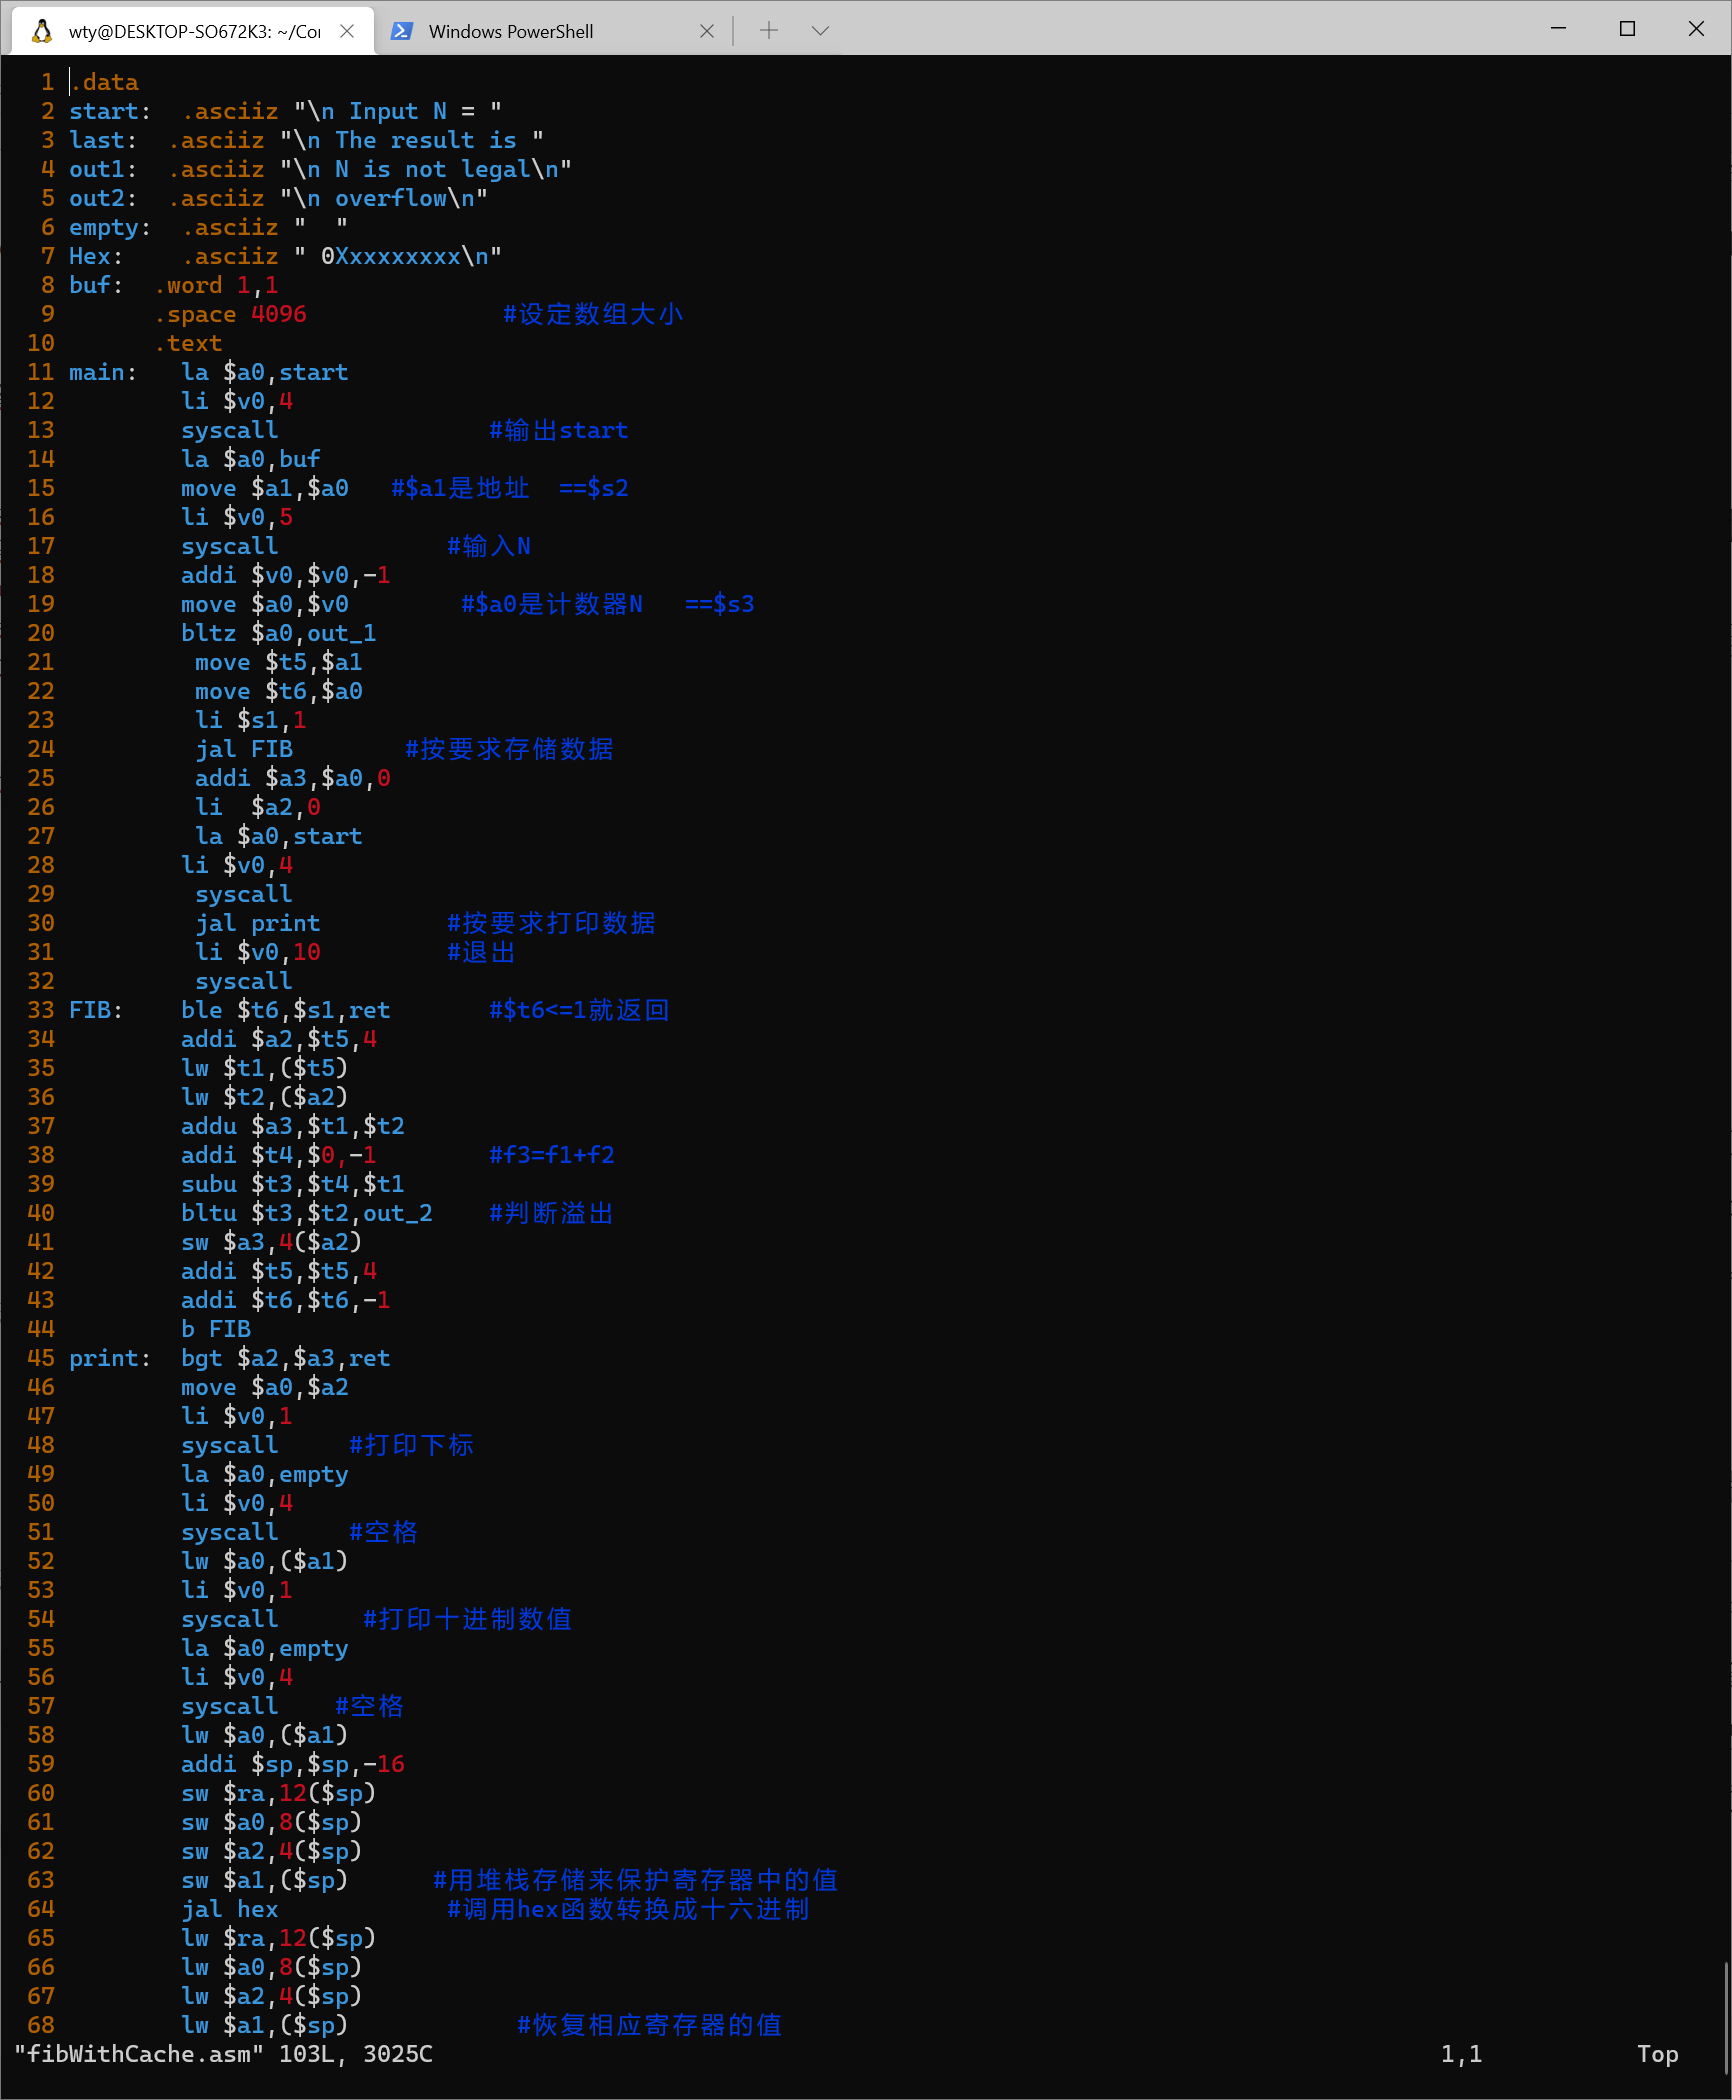
\includegraphics[width=\textwidth]{figures/figure3.png}
	\caption{处理过的汇编代码截图}
	\label{fig:ExtraProCSource2}
\end{figure}
\section{加分项二}

\section{总结}
这里总结全文。


% \section{习题环境}

% \begin{exs}
% 请证明勾股定理。
% \end{exs}
% \begin{proof}
% 这是证明。末尾后会自动添加方块以示结束。
% \end{proof}

% \begin{exs}
% 请计算 $1+2+\ldots +100$。
% \end{exs}
% \begin{proof}[解答]
% 这是解答。末尾后会自动添加方块以示结束。
% \end{proof}

\newpage

\begin{thebibliography}{9}

\addcontentsline{toc}{section}{参考文献}  % 目录中加入参考文献

\bibitem{cao17}
  Rongmei Cao.
  Matrix Theory.
  Nanjing University of Aeronautics and Astronautics, 2017.  

\bibitem{pbrs14}
  Perozzi, Bryan, R. Al-Rfou, and S. Skiena. "DeepWalk: online learning of social representations." (2014):701-710.

\bibitem{czw17}
  李彦冬, 郝宗波, and 雷航. "卷积神经网络研究综述." 计算机应用 36.9(2016):2508-2515.
\bibitem{DongShouCPU}
  雷思磊, 自己动手写CPU
\end{thebibliography}

\end{document}
